% ------------------------------------------------------------------------------------
\section{Ejercicio 1}
\textbf{(Problema en ecología)} Sean $X_{1}, \ldots X_{m}$ variables aleatorias donde $X_{i}$ denota el número de individuos de una especie en cierta región. Suponga que $X_{i} | N, p \sim Binom(N, p)$, entonces
	\begin{equation} \label{eq:1}
		f(\bar{x} \mid N, p)=\prod_{i=1}^{m} \frac{N!}{x_{i}!\left(N-x_{i}\right)!} p^{x_{i}}(1-p)^{N-x_{i}} .
	\end{equation}
	
	Asumiendo la distribución a priori $p \sim Beta(\alpha, \beta)$ y $N \sim h(\cdot)$, donde $h$ es una distribución discreta en $\left\{0,1,2, \dots, N_{\max }\right\}$, se tiene definida la distribución posterior $f(N, P \mid \bar{x})$.
	
	A partir del algoritmo MH, simule valores de la distribución posterior usando un kernel híbrido. Para ello considere \textbf{como sugerencia} la 
	siguiente distribución inicial para el MCMC
	\begin{equation}\label{eq:2}
		p \sim \mathrm{U}(0,1) \quad \text { y } \quad N \sim \mathrm{U}_{d}\left\{\max _{i \in\{1, \ldots, m\}}\left(x_{i}\right), \max _{i \in\{1, \ldots, m\}}\left(x_{i}\right)+1, \ldots, N_{\max }\right\}
	\end{equation}
	y las propuestas
	\begin{itemize}
		\item \underline{Propuesta 1:} De la condicional total de $p$ (kernel Gibbs).
		\item \underline{Propuesta 2:} De la a priori.
		\item \underline{Propuesta 3:} Propuesta hipergeométrica (¿?).
		\item \underline{Propuesta 4:} Poisson: $N_{p} \sim \max _{i \in\{1, \ldots, m\}}\left(x_{i}\right)+$ Poisson(?).
		\item \underline{Propuesta 5:} Caminata aleatoria
	\end{itemize}
	\begin{equation} \label{eq:3}
		N_{p}=N+\epsilon, \quad \mathbb{P}(\epsilon=1)=\frac{1}{2}=\mathbb{P}(\epsilon=-1)
	\end{equation}
	
	Los datos son estos: $7,8,6,5,2,8,6,6,7,4,8,8,6,4,8,8,10,5,4,2$.
	
	A priori, esperamos que sea difícil observar a los individuos entonces $\alpha=1$, $\beta=20$. La especie no es muy abundante y entonces $N_{\max }= 1000$ y $h(N)=1 /\left(N_{\max }+1\right)$; $N \in\left\{0,1,2, \ldots, N_{\max }\right\}$.
	
	Las propuestas y distribución inicial para el MCMC de arriba son \textbf{solamente sugerencia}, propongan otras propuestas, experimenten y comenten.

\vspace{5mm}
{\color{gray} \hrule}
\vspace{5mm}
\textcolor{BrickRed}{\it Respuesta:}

Sabemos que la verosimilitud conjunta de los datos observados $\bar{x}$ está dada por \eqref{eq:1} y se asume que $p$ tiene una distribución a priori beta:
\begin{equation} \label{eq:4}
	p \sim Beta (\alpha, \beta),
\end{equation}
donde $\alpha = 1$  y  $\beta = 20$, lo que refleja una creencia previa de que $p$ es pequeño (dificultad para observar individuos). Además, se asume que $N$ sigue una distribución uniforme discreta en el rango $[0, 1, \dots, N_{\max} = 1000]$:
\begin{equation} \label{eq:5}
	h(N) = \frac{1}{N_{\max} + 1}.
\end{equation}

La inferencia bayesiana se basa en calcular la distribución posterior de los parámetros $N$ y $p$ dados los datos observados $\bar{x}$. Por el teorema de Bayes:
\begin{equation} \label{eq:6}
	\begin{aligned}
		f(N, p \mid \bar{x}) 
		&\propto f(\bar{x} \mid N, p) \cdot h(N) \cdot Beta (p; \alpha, \beta)\\
	\end{aligned}
\end{equation}
donde:
\begin{itemize}
	\item $f(\bar{x} \mid N, p)$: Verosimilitud conjunta de los datos.
	\item $h(N)$: Prior de $N$ (notemos que la distribución no depende explícitamente de $N$).
	\item $Beta (p; \alpha, \beta)$: Prior de $p$.
\end{itemize}

Reescribiendo \eqref{eq:6}, se tiene
\begin{equation}\label{eq:7}
	\begin{aligned}
		f(N, p &\mid \bar{x}) \propto f(\bar{x} \mid N, p) \cdot h(N) \cdot Beta (p; \alpha, \beta) \propto  f(\bar{x} \mid N, p) \cdot Beta (p; \alpha, \beta)\\
		& \propto \prod_{i=1}^m \binom{N}{x_i} \cdot p^{\sum x_i} (1-p)^{mN - \sum x_i} \cdot  p^{\alpha - 1} (1-p)^{\beta - 1} \cdot \mathbbm{1}_{\{0,\dots,N\}} (x_i) \mathbbm{1}_{\{0,\dots,N_{max}\}} (N) \mathbbm{1}_{(0,1)} (p)\\
		& \propto \prod_{i=1}^m \binom{N}{x_i} \cdot p^{\alpha + \sum x_i - 1} (1-p)^{\beta + mN - \sum x_i - 1} \cdot \mathbbm{1}_{\{0,\dots,N\}} (x_i) \mathbbm{1}_{\{0,\dots,N_{max}\}} (N) \mathbbm{1}_{(0,1)} (p).
	\end{aligned}
\end{equation}
Podemos notar que esto es proporcional a una distribución
\begin{equation} \label{eq:8}
	Beta \left(\alpha + \sum x_i, \quad \beta + mN - \sum x_i  \right)
\end{equation}
para $p$ dado $N$, la cual se puede usar como una propuesta Gibbs.

\newpage
En el archivo \textcolor{mediumblue}{ejercicio1\_tarea9.py} se implementa la función 
\begin{center}
	\textit{METROPOLIS\_HASTINGS\_HYBRID\_KERNELS()},
\end{center}
la cual aplica el algoritmo Metropolis-Hastings con kérneles híbridos para $K$ propuestas simulando una cadena de Markov en $\mathbb{R}^n$ y toma los siguientes argumentos:
\begin{itemize}
	\item La función objetivo $f$ (para este ejercicio, se trata de la distribución posterior dada en \eqref{eq:6}).
	\item Una lista de las $K$ funciones que generan las propuestas $[q_{1_{gen}}, \dots, q_{K_{gen}}]$.
	\item Lista de las $K$ funciones que calculan la densidad de probabilidad de las propuestas $[q_{1_{pdf}}, \dots, q_{K_{pdf}}]$. Es importante que se respete el mismo orden de la lista de funciones generadoras.
	\item Lista de las $K$ probabilidades de seleccionar cada kernel de propuesta $[p_1,\dots,p_{K}]$. Es importante que se respete el mismo orden de la lista de funciones generadoras y que $\sum_{k} p_k =1$. Si esta lista no se da, se toman probabilidades iguales para cada kernel, i.e., $p_1=\cdots = p_K = \frac{1}{K}$.
	\item El valor inicial $x_0$ en el soporte de la distribución objetivo.
	\item El número de iteraciones del algoritmo (casi siempre se usa $N = 10,000$).
\end{itemize}

La función regresa la cadena simulada en $\mathbb{R}^n$ e imprime la tasa de aceptación lograda y el conteo de aceptaciones por kernel.

A continuación, se implementa la función \textit{posterior()} descrita por \eqref{eq:6}, que es nuestra distribución objetivo. Notemos que no se considera explícitamente la distribución $h(N)$ ya que la densidad $\frac{1}{N_{\max} + 1}$ no depende explícitamente de $N$ y se considera como constante de proporcionalidad.

\textbf{Distribución inicial:}
\begin{equation}\label{eq:9}
	N \sim \mathrm{U}_{d}\left\{\max _{i \in\{1, \ldots, m\}}\left(x_{i}\right), \max _{i \in\{1, \ldots, m\}}\left(x_{i}\right)+1, \ldots, \max _{i \in\{1, \ldots, m\}}\left(x_{i}\right) + r\right\} \text{ y } p\sim U(0,1).
\end{equation}
El ejercicio propone tomar como distribuciones iniciales a las dadas en la expresión \eqref{eq:2}. Debido a los buenos resultados en la mayoría de los experimentos, se tomó la decisión de mantener la distribución inicial de $p\sim U(0,1)$, sin embargo, se decidió cambiar la de $N$ ya que el intervalo discreto $[x_{max} = 10,\dots, N_{max} = 1000]$ es demasiado grande y de vez en cuando generaba saltos muy grandes en los valores iniciales de $N$. En su lugar se tomó la distribución inicial de $N$ como vemos en \eqref{eq:9} para $r<N_{max}$, elegible por el usuario (en este caso nos quedamos con $r=120$). Esta distribución se implementa en la función \textit{initial\_distribution()} en el archivo \textcolor{mediumblue}{ejercicio1\_tarea9.py}

\textbf{Propuestas:}

En el archivo \textcolor{mediumblue}{ejercicio1\_tarea9.py}, se implementan las propuestas (\textit{prop$i$\_gen()}), así como su densidad de probabilidad respectiva (\textit{prop$i$\_pdf()}) y estas se describen a continuación. Inicialmente, se consideraron las propuestas dadas por el ejercicio mismo, pero experimentando con cada una y con la compatibilidad entre ellas, se realizaron los siguientes cambios que evitaron indeterminaciones y tuvieron resultados satisfactorios, aunque no únicos.

\begin{itemize}
	\item \underline{Propuesta 1:} 	Kérnel Gibbs para $p$ dado $N$.
	\begin{equation} \label{eq:10}
		p\sim Beta \left(\alpha + \sum x_i, \quad \beta + mN - \sum x_i  \right) \text{ y } N \text{ fijo.}
	\end{equation}
\end{itemize}
Se define la función \textit{prop1\_gen()} que implementa la distribución Gibbs (distribución condicional completa de $p$ dado $N$ y los datos $\bar{x}$) descrita en \eqref{eq:8} y \eqref{eq:10} siendo cuidadosos con el soporte de esta distribución ya que el parámetro $\beta + mN - \sum x_i$ debe ser positivo. En caso de que no, se propone $p\sim Beta (\alpha + \sum x_i, 1)$. También se define su densidad de probabilidad en la función \textit{prop1\_pdf()}. Se eligió conservar esta propuesta ya que un paso de Gibbs siempre acepta la propuesta porque la muestra proviene de la distribución condicional verdadera. Esto asegura exploración eficiente en la dimensión de $p$.

\begin{itemize}
	\item \underline{Propuesta 2:} Propuesta independiente y a priori para $p$.
	\begin{equation} \label{eq:11}
		N \sim \mathrm{U}_{d}\left\{x_{max}, \dots, x_{max} + r\right\} \text{ y } p\sim Beta(\alpha=1, \beta = 20).
	\end{equation}
\end{itemize}
El ejercicio recomienda usar como propuesta a las a prioris, sin embargo, dado que la distribución a priori de $N$ es $h(N)=\frac{1}{1001}$, se tendrá una tasa de aceptación demasiado baja para cada valor propuesto. Por esto, se eligió usar a la distribución inicial para $N$ dada por \eqref{eq:9} para poder controlar la nueva probabilidad $h(N)=\frac{1}{r}$ con el valor de $r$ (en particular, se tomó $r = 120$ ya que tuvo un buen desempeño). En cambio, para $p$ se mantuvo la propuesta a priori: $p\sim Beta(\alpha=1, \beta = 20)$. La función generadora y su función de densidad se definen en \textit{prop2\_gen()} y \textit{prop2\_pdf()} respectivamente. Se eligió esta propuesta, ya que, dado que es una propuesta independiente, introduce aleatoriedad independiente de los datos, lo que ayuda a evitar que la cadena quede atrapada en un modo local y permite exploración de regiones remotas del espacio de parámetros, fomentando una mejor cobertura de la posterior.

\begin{itemize}
	\item \underline{Propuesta 3:} Propuesta hipergeométrica.
	\begin{equation} \label{eq:12}
		N \sim Hipergeom(M = N_{max}, n = \sum x_{i}, N = m) \text{ y } p \text{ fijo.}
	\end{equation}
\end{itemize}
Se está modelando el tamaño poblacional $N$ como una variable que sigue una distribución hipergeométrica. Los parámetros específicos son: $M = N_{max}$ ya que es el tamaño de la población máxima posible, $n = \sum x_{i}$ es el número total de éxitos en los datos observados y $N = m$ corresponde al número de datos observados. Se escogió de esta forma ya que los datos observados ($\sum x_i$  éxitos en $m$ observaciones) sugieren que $N$ debe estar acotado entre el valor máximo observado en los datos y $N_{max}$. La distribución hipergeométrica respeta esta restricción y se está trabajando con un conjunto finito de datos observados, que podemos considerar como una muestra extraída sin reemplazo de una población más grande. La función generadora y su función de densidad se definen en \textit{prop3\_gen()} y \textit{prop3\_pdf()} respectivamente.

\begin{itemize}
	\item \underline{Propuesta 4:} Poisson.
	\begin{equation} \label{eq:13}
		N_{p} \sim \max _{i \in\{1, \ldots, m\}}\left(x_{i}\right)+ Poisson(\lambda) \text{ y } p \text{ fijo.}
	\end{equation}
\end{itemize}
Esta propuesta tuvo diversas variantes al momento de experimentar con ella. Inicialmente se consideró tomar el parámetro $\lambda=Np$ ya que, como sabemos, si $N$ es grande y $p$ pequeño, entonces $Poisson(Np)$ se comporta como una binomial con parámetros $(N,p)$, que es exactamente lo que nos interesa. Sin embargo, causaba muchos problemas al momento de correr el algoritmo, debido a que se veía mucha variabilidad en los valores de $N$ y $p$, esto se observó al momento de generar las gráficas ya que se veía una posterior multimodal y no se observaba un buen ajuste a los datos (ver figuras siguientes).

Con la intención de tener una propuesta no independiente para $N$, también se consideró usar $\lambda = N$ ya que parecía una buena propuesta debido a que restringe la exploración de $N$ a valores realistas y permite una transición más suave entre valores cercanos de $N$. Sin embargo, sucedían cosas similares al caso $\lambda=Np$, además de indeterminaciones y una tasa de aceptación bastante baja.

Finalmente, se decidió conservar una tasa $\lambda$ constante. Esto permite ajustar el parámetro $\lambda$ explícitamente, proporcionando control sobre la dispersión de $N$. en particular, se tomó $\lambda = 400$ ya que tuvo un buen desempeño, pero cualquier valor alrededor de este, funciona bien. La función generadora y su función de densidad se definen en \textit{prop4\_gen()} y \textit{prop4\_pdf()} respectivamente.

\begin{itemize}
	\item \underline{Propuesta 5:} Caminata aleatoria.
	\begin{equation}\label{eq:14}
		N_p = N + \epsilon, \quad \text{donde } \epsilon \sim \{-1, 1\} \text{ y } p \text{ fijo.}
	\end{equation}
\end{itemize}
Se decidió conservar esta propuesta ya que en cadenas de Markov, las propuestas simples y simétricas (caminatas aleatorias) son robustas para exploración local y garantizan una tasa de aceptación razonable. Sin embargo, su convergencia puede ser lenta si la posterior es amplia, pero para ese caso, ya se cuentan con otras propuestas que cuentan con más variabilidad. La función generadora y su función de densidad se definen en \textit{prop5\_gen()} y \textit{prop5\_pdf()} respectivamente.

\textbf{Conclusión general de las propuestas:}

Las propuestas $1$ y $3$ son informativas (dependen de los datos), lo que fomenta una exploración más dirigida. Las propuestas $2$, $4$ y $5$ son más exploratorias, permitiendo cobertura global del espacio de parámetros. Las propuestas Gibbs y hipergeométrica aseguran explotación local eficiente, mientras que las propuestas uniformes y Poisson permiten escapar de nodos locales, promoviendo una mejor mezcla.

Por el Teorema de convergencia, sabemos que la cadena converge a la distribución posterior si:
\begin{itemize}
	\item La cadena es irreducible (puede alcanzar cualquier estado en su espacio de parámetros).
	\item La cadena es aperiódica (no tiene ciclos regulares).
	\item Las propuestas son ergódicas (cubren todo el soporte de la posterior).
\end{itemize}
Y la elección de propuestas satisface estas condiciones porque:
\begin{itemize}
	\item Hay propuestas que exploran globalmente ($2$, $4$ y $5$).
	\item Hay propuestas que exploran localmente ($1$ y $3$).
	\item Todas las propuestas respetan las restricciones del soporte.
\end{itemize}
Cada propuesta tiene un rol específico en garantizar una buena mezcla y convergencia. Además, su combinación fomenta una cobertura eficiente del espacio de parámetros, lo que resulta en estimaciones robustas de la posterior, como se ve a continuación:

\textbf{Resultados:}

Con ayuda de las funciones auxiliares descritas en \ref{sec:funauc} e implementadas en \textcolor{mediumblue}{funciones\_auxiliares.py}, se puede visualizar los resultados generados. Se ejecuta el código principal, en el cual se definen los datos a tratar, así como los parámetros para la distribución posterior, la a priori, la inicial y las propuestas. Para el algoritmo Metropolis-Hastings se realizaron $10000$ muestras y el punto inicial resultó ser $[38, 0.2795]$ (se usó una semilla para la reproducibilidad de los resultados).

A continuación, se definieron las listas de funciones generadoras de cada propuesta, así como de sus respectivas funciones de densidad y a todas las propuestas se les dio probabilidad de elección igual a $\frac{1}{6}$. Al generar la cadena, se obtuvo un $42.77\%$ de aceptación de propuestas y con ayuda de la función \textit{estim\_burn\_in\_and\_modes()} se calcularon las modas resultantes de cada parámetro y el burn-in a considerar:
\begin{itemize}
	\item Moda de $N$: $408$,
	\item Moda de $p$: $0.0151$,
	\item Burn-in: $538$.
\end{itemize}

A continuación se tienen los histogramas de las cadenas de Markov simuladas. Además, grafica el histograma de los datos y las
distribución binomial estimada, marcando las modas calculadas en cada caso. Vemos que el ajuste es relativamente bueno debido a que se cuenta con muy pocos datos.
\begin{figure}[h!]
	\centering
	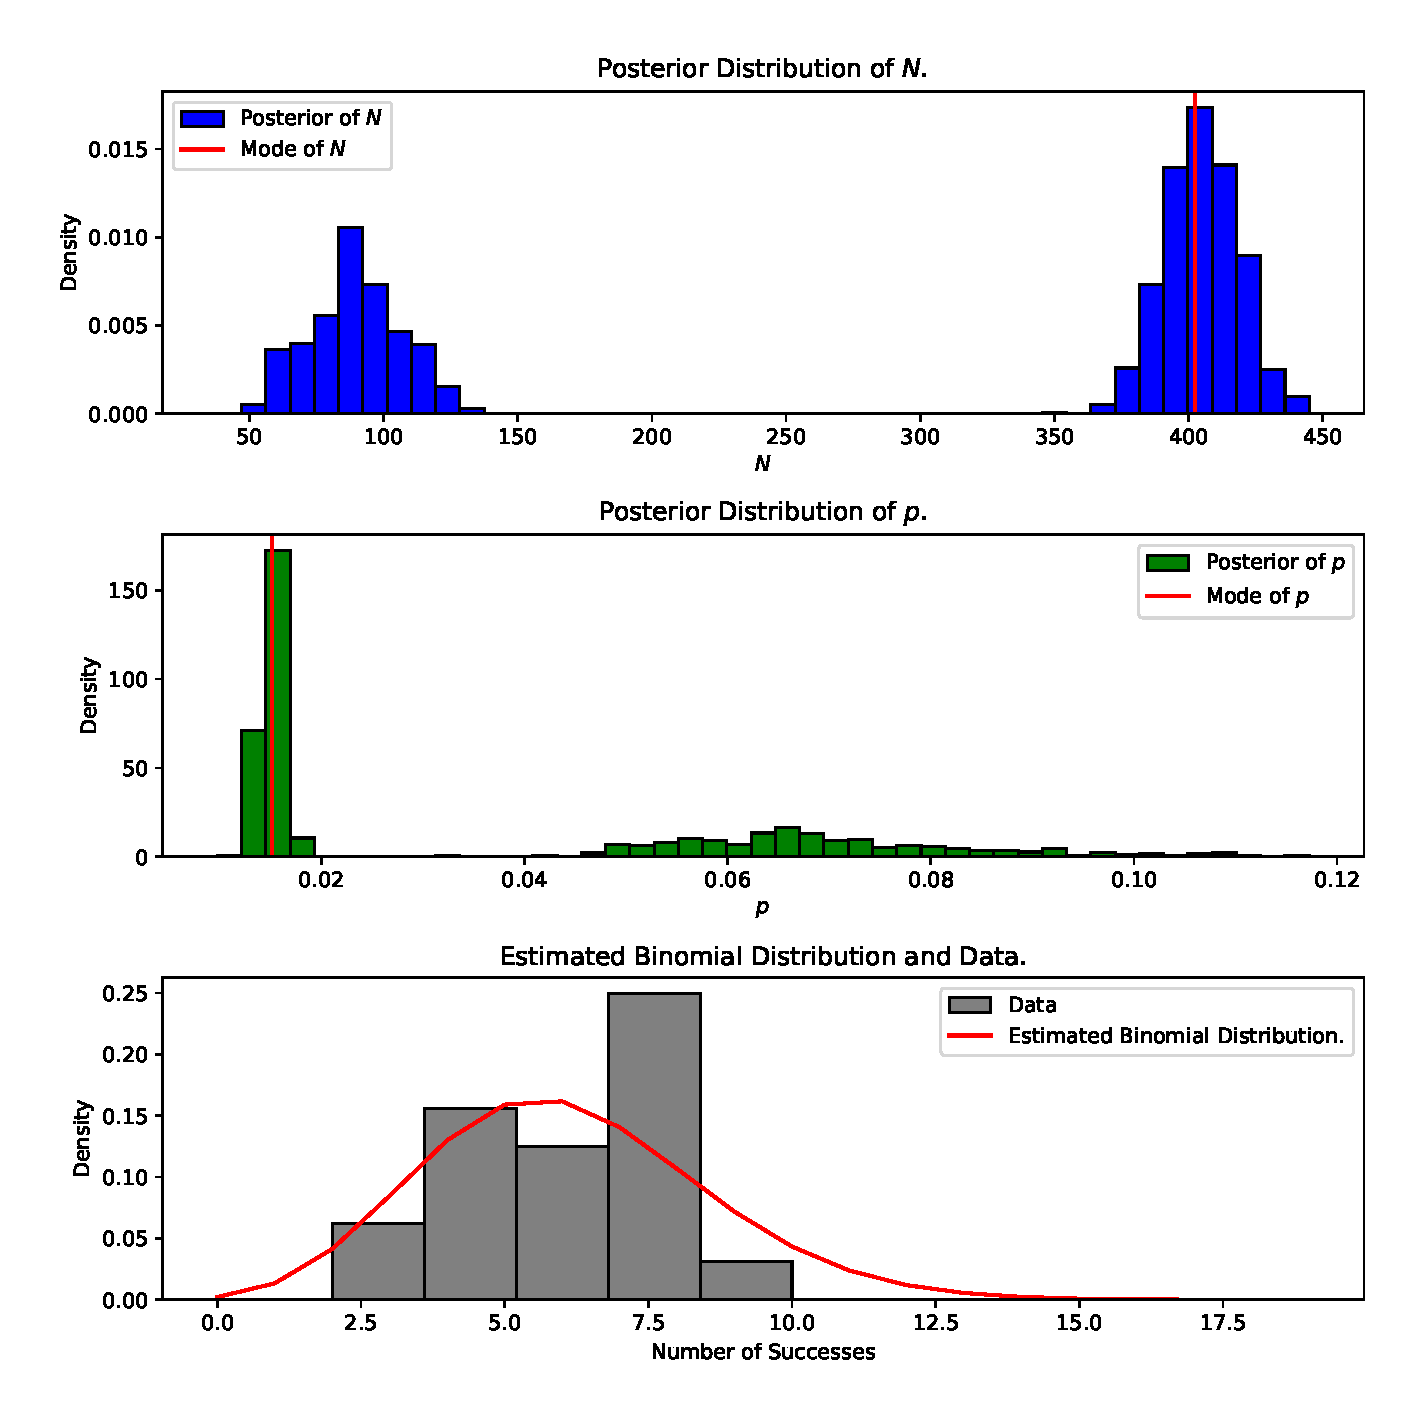
\includegraphics[width=0.8\textwidth]{IMAGENES/histogram_ex1.pdf}
\end{figure}

A continuación, se tiene la evolución de las cadenas de Markov marginales con respecto al burn-in estimado.
\begin{figure}[h!]
	\centering
	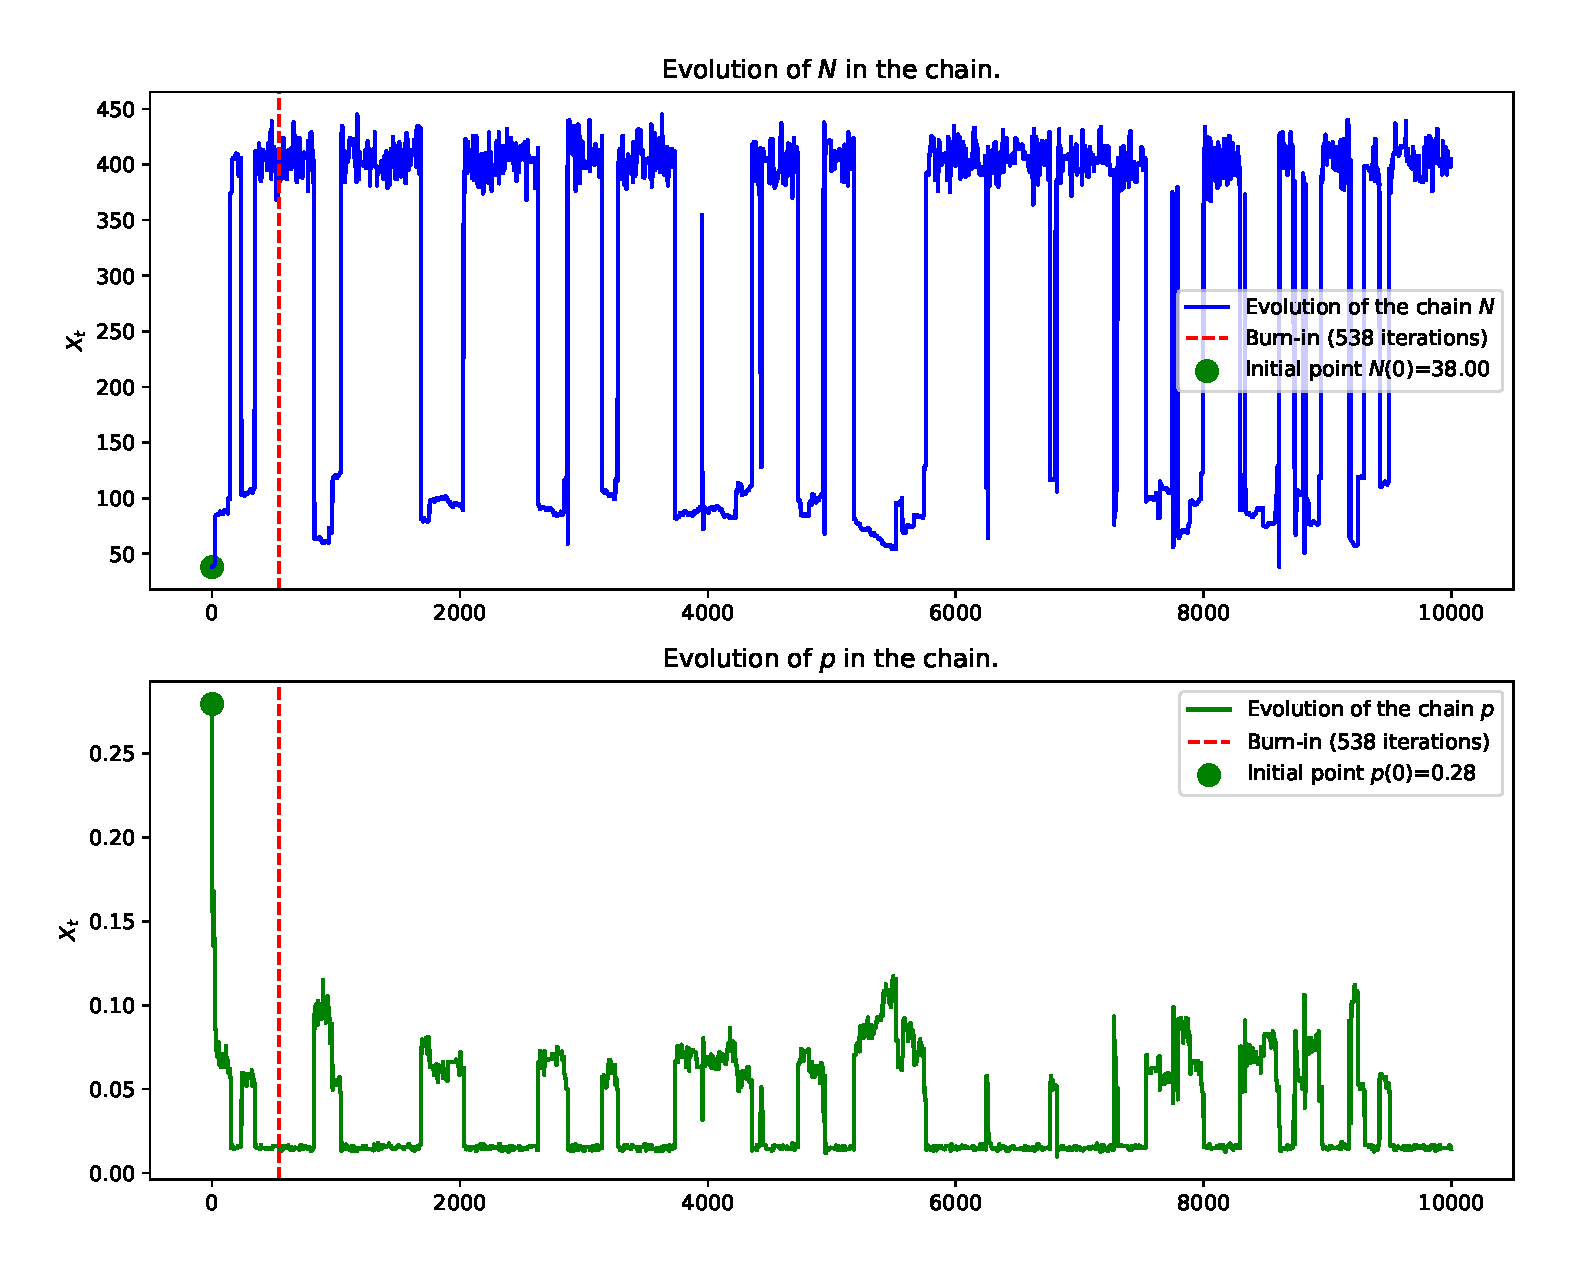
\includegraphics[width=0.8\textwidth]{IMAGENES/marginal_evolution_ex1.pdf}
\end{figure}

Finalmente, se tiene la trayectoria de la cadena de Markov en el espacio de parámetros.
\begin{figure}[h!]
	\centering
	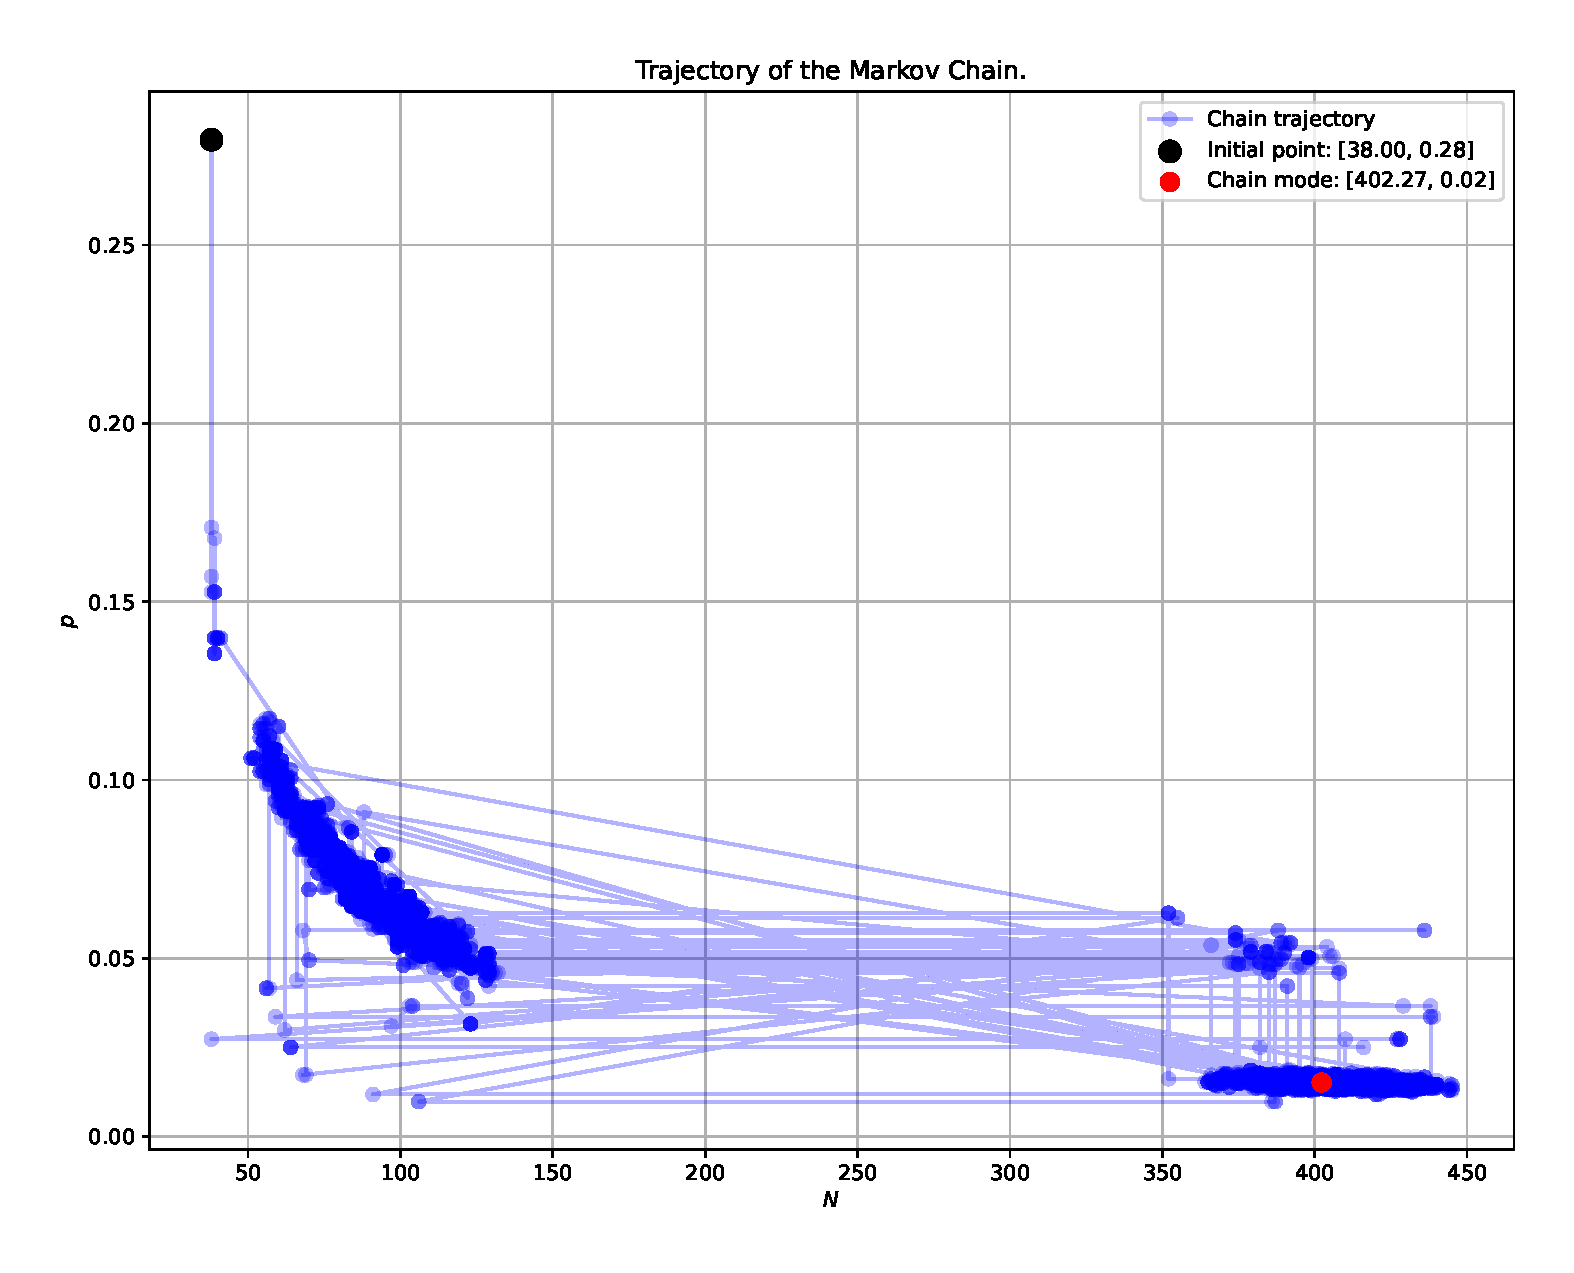
\includegraphics[width=0.85\textwidth]{IMAGENES/trayectory_ex1.pdf}
\end{figure}

Al observar los resultados y el comportamiento de las gráficas, se puede notar que en el histograma de $N$, existe un pico pronunciado en valores altos alrededor de $408$, que corresponde a la moda de la distribución posterior. Esto sugiere que el MCMC identificó esta región como el valor más probable para $N$. Por otro lado, la moda de $p$ se encuentra alrededor de $0.02$, lo que indica que, al incrementar $N$, el modelo ajusta $p$ a valores más pequeños para mantener la consistencia con los datos observados, reflejando un efecto compensatorio entre ambos parámetros.

La trayectoria de la cadena refuerza esta observación, mostrando que la mayor parte de la exploración se concentra cerca de $N\approx 408$ y $p \approx 0.02$. Sin embargo, al inicio del muestreo, se exploraron combinaciones diferentes, caracterizadas por valores más bajos de $N$ y valores más altos de $p$. Esto indica que el espacio de parámetros admite múltiples combinaciones compatibles con los datos observados, aunque el MCMC finalmente converge hacia la región de mayor probabilidad.

Este comportamiento puede atribuirse a la poca cantidad de datos disponibles, lo que reduce la capacidad del modelo para discriminar entre combinaciones de $N$ y $p$ ya que, para distintos valores de los parámetros de las propuestas como $\lambda$ o $r$, se observaba este fenómeno de "buen" ajuste de la posterior para distintos valores de $N$ y $p$. Se optó por estas versiones ya que hubo pocos problemas en la implementación y poca variabilidad en las trayectorias de la cadena.

